\subsection*{Memory Cell Architecture}
At the microscopic level, NAND flash memory consists of floating-gate transistors arranged in a three-dimensional grid structure. 
Each cell stores data by trapping electrons in the floating gate, which changes the threshold voltage of the transistor. When the 
controller reads the cell, it measures this voltage to determine whether the cell represents a binary 1 or 0.

Modern NAND flash has evolved to store multiple bits per cell through careful voltage level management. Single-level cell (SLC) 
technology stores one bit per cell, offering the highest performance and endurance. Multi-level cell (MLC) technology stores two 
bits per cell, Triple-level cell (TLC) stores three bits, and Quad-level cell (QLC) stores four bits per cell.

As we increase the number of bits per cell, we achieve higher storage density and lower cost per gigabyte, but with trade-offs in 
performance and endurance. This is why different applications benefit from different NAND types — enterprise workloads often prefer 
SLC or MLC for reliability, while consumer applications typically use TLC or QLC for cost-effectiveness.
\cite{lexar_nvme}
\begin{figure}[H]
    \centering
     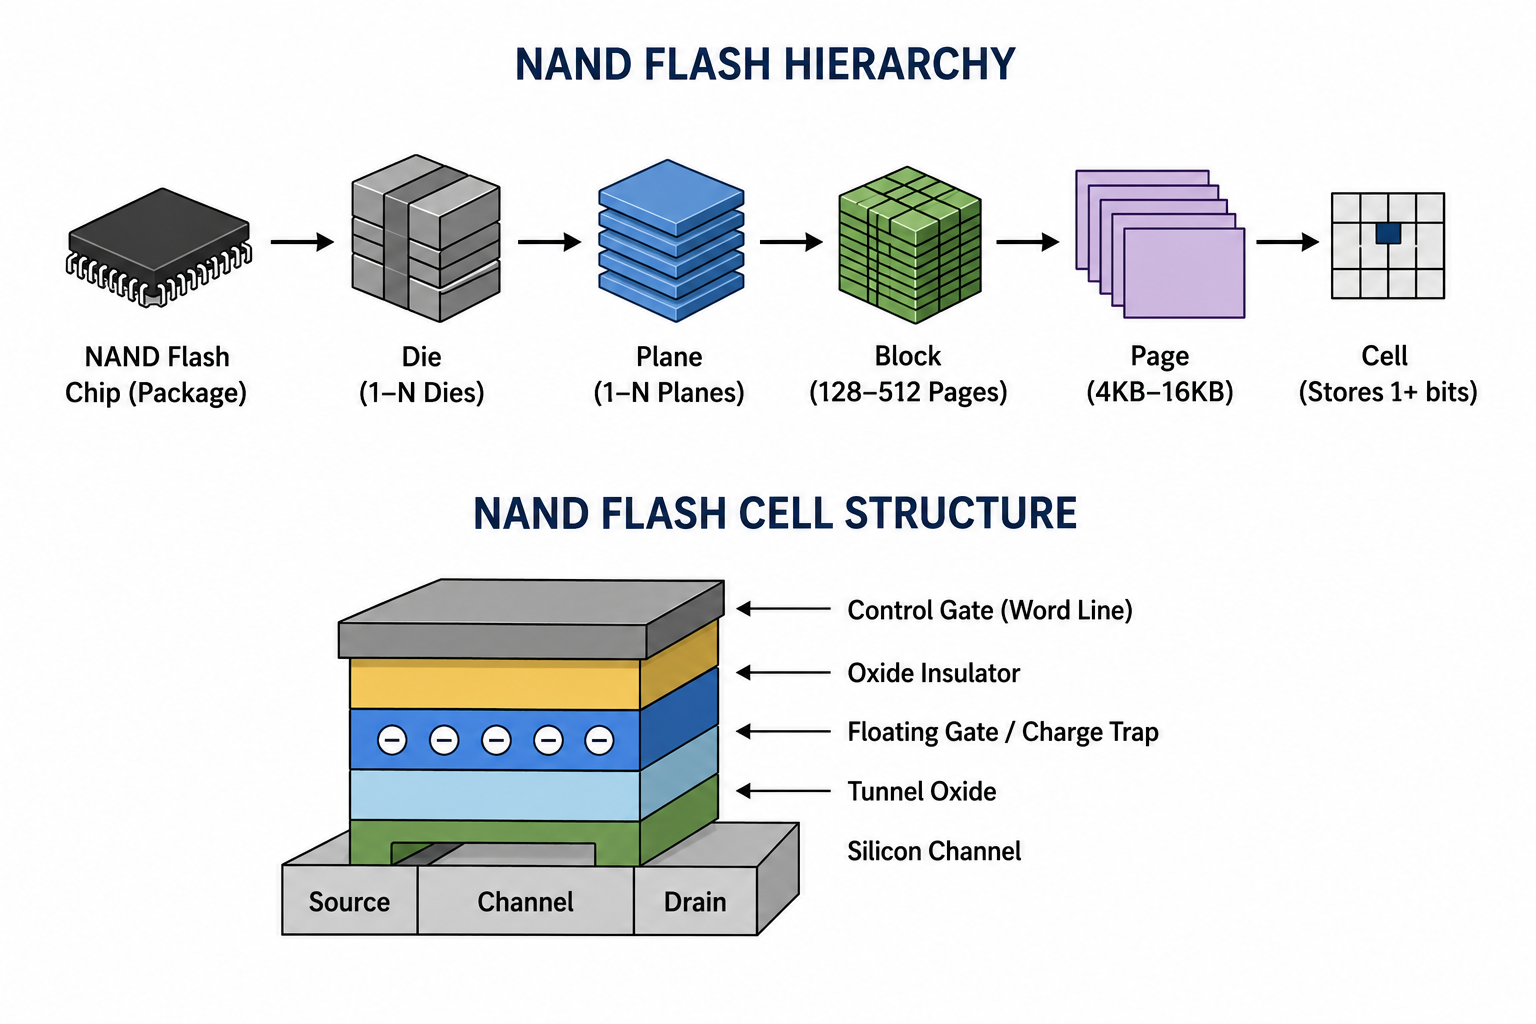
\includegraphics[width=0.7\textwidth]{Nand flash cell.png}
    \caption{Memory Cell Architecture }
    \label{fig: nvme cell } 
\end{figure}